\documentclass{article}

\usepackage[preprint]{neurips_2026}

\usepackage[utf8]{inputenc}
\usepackage[T1]{fontenc}
\usepackage{hyperref}
\usepackage{url}
\usepackage{booktabs}
\usepackage{amsfonts}
\usepackage{amsmath}
\usepackage{nicefrac}
\usepackage{microtype}
\usepackage{xcolor}
\usepackage{graphicx}

\title{Measurement-Theoretic Active Elicitation for Predicting AI
Evaluation Outcomes}

\author{%
  Dinesh Katupputhur Ramprasath \\
  Stanford University \\
  \texttt{din1993@stanford.edu} \\
}

\begin{document}

\maketitle

\begin{abstract}
Predicting whether an AI system answers a benchmark item correctly, under a
strict budget on how many ground-truth labels may be purchased, is a
measurement problem in disguise: the correctness probability is a Rasch
interaction between a subject's latent \emph{ability} and an item's
\emph{difficulty}, and the choice of which labels to buy is the efficient,
Fisher-information-guided elicitation problem of adaptive testing. We recast the
NeurIPS~2026 Predictive AI Evaluation Competition in this frame and contribute
(i) a Bayesian item-response predictor whose posterior over subject ability is
updated online as labels arrive, giving calibrated uncertainty where our
black-box tabular baseline has none, and (ii) a Fisher-information /
expected-Brier-reduction acquisition policy that replaces an ad-hoc uncertainty
heuristic and directly targets the competition's area-under-the-Brier-curve
(ALC) metric. On a controlled Rasch world and on a genuine response matrix of
119 AI systems over 1{,}531 items reconstructed from our competition's logged
outcomes, evaluated by an offline replay harness with bootstrap confidence
intervals, we find a clear split: the Bayesian predictor recovers latent ability (correlation $0.83$) and its uncertainty-marginalised
output is better calibrated and lower-Brier than a plug-in point estimate
(ECE $0.028$ vs $0.041$). Information-directed acquisition pins ability down far
faster than random selection (ability error at budget 7 of $0.44$--$0.49$ vs
$0.72$), but this advantage \emph{largely washes out} in Brier ALC: across all
three datasets the four policies lie within each other's $95\%$ confidence
intervals. We conclude --- consistent with our pre-registered null analysis ---
that under a well-calibrated, uncertainty-aware predictor the label-selection
policy is second-order for Brier ALC; the predictor, not the policy, is where
the gains lie.
\end{abstract}

\section{Introduction and Background}

\paragraph{The task.} The NeurIPS~2026 Predictive AI Evaluation Competition asks
a predictor to output $P(\text{subject answers item correctly})$ for
\mbox{(subject, item)} pairs, where a \emph{subject} is an AI system under fixed
evaluation settings and an \emph{item} is a benchmark task. It is a streaming
test-time adaptation problem: for each subject--benchmark pair the predictor may
purchase ground-truth labels under the nested budget schedule
$\{0,1,3,7,15,31\}$, and is scored by \textbf{Brier~ALC} --- the
budget-weighted area under the Brier learning curve, weights
$(0.1,0.2,0.2,0.2,0.2,0.1)$. Lower is better; a constant $0.5$ predictor scores
$0.25$.

\paragraph{Two coupled problems.} The task decomposes into \emph{estimation} ---
predicting a latent ``will this subject get this item right,'' a Rasch
interaction $\sigma(\theta_s - \beta_i)$ between subject ability $\theta_s$ and
item difficulty $\beta_i$ --- and \emph{elicitation} --- choosing which labels
to buy under a budget to drive Brier down fastest, which is efficient
Fisher-information elicitation / adaptive testing.

\paragraph{Motivation from our prior submissions.} Over 18 competition
submissions (best Brier~ALC $0.162$, a tabular in-context model with text
embeddings), two structural weaknesses remained, both in the scope of
measurement science. First, the predictor is a black box: we fit a tabular model
on acquired labels and blend toward a hand-coded prior with a linear trust
weight $\min(n/10,1)$, with no latent-trait model and no posterior over ability,
so we cannot reason about how much a label will help before buying it. Second,
acquisition is a one-line heuristic that buys a label whenever
$|\hat p - 0.5|\le 0.20$ --- a crude proxy for informativeness that ignores how
much a label transfers to the frozen evaluation pool and ignores the budget
schedule, yet acquisition is what ALC rewards most.

\paragraph{Research questions.}
\textbf{(RQ1)} Does a Bayesian IRT predictor match or beat the black-box tabular
predictor on Brier while providing calibrated uncertainty?
\textbf{(RQ2)} Does a Fisher / expected-Brier-reduction acquisition policy beat
the $|\hat p - 0.5|$ heuristic and random acquisition at equal budget?
\textbf{(RQ3)} How much of the ALC gain comes from a better cold-start prior
versus better acquisition?

\begin{figure}[t]
  \centering
  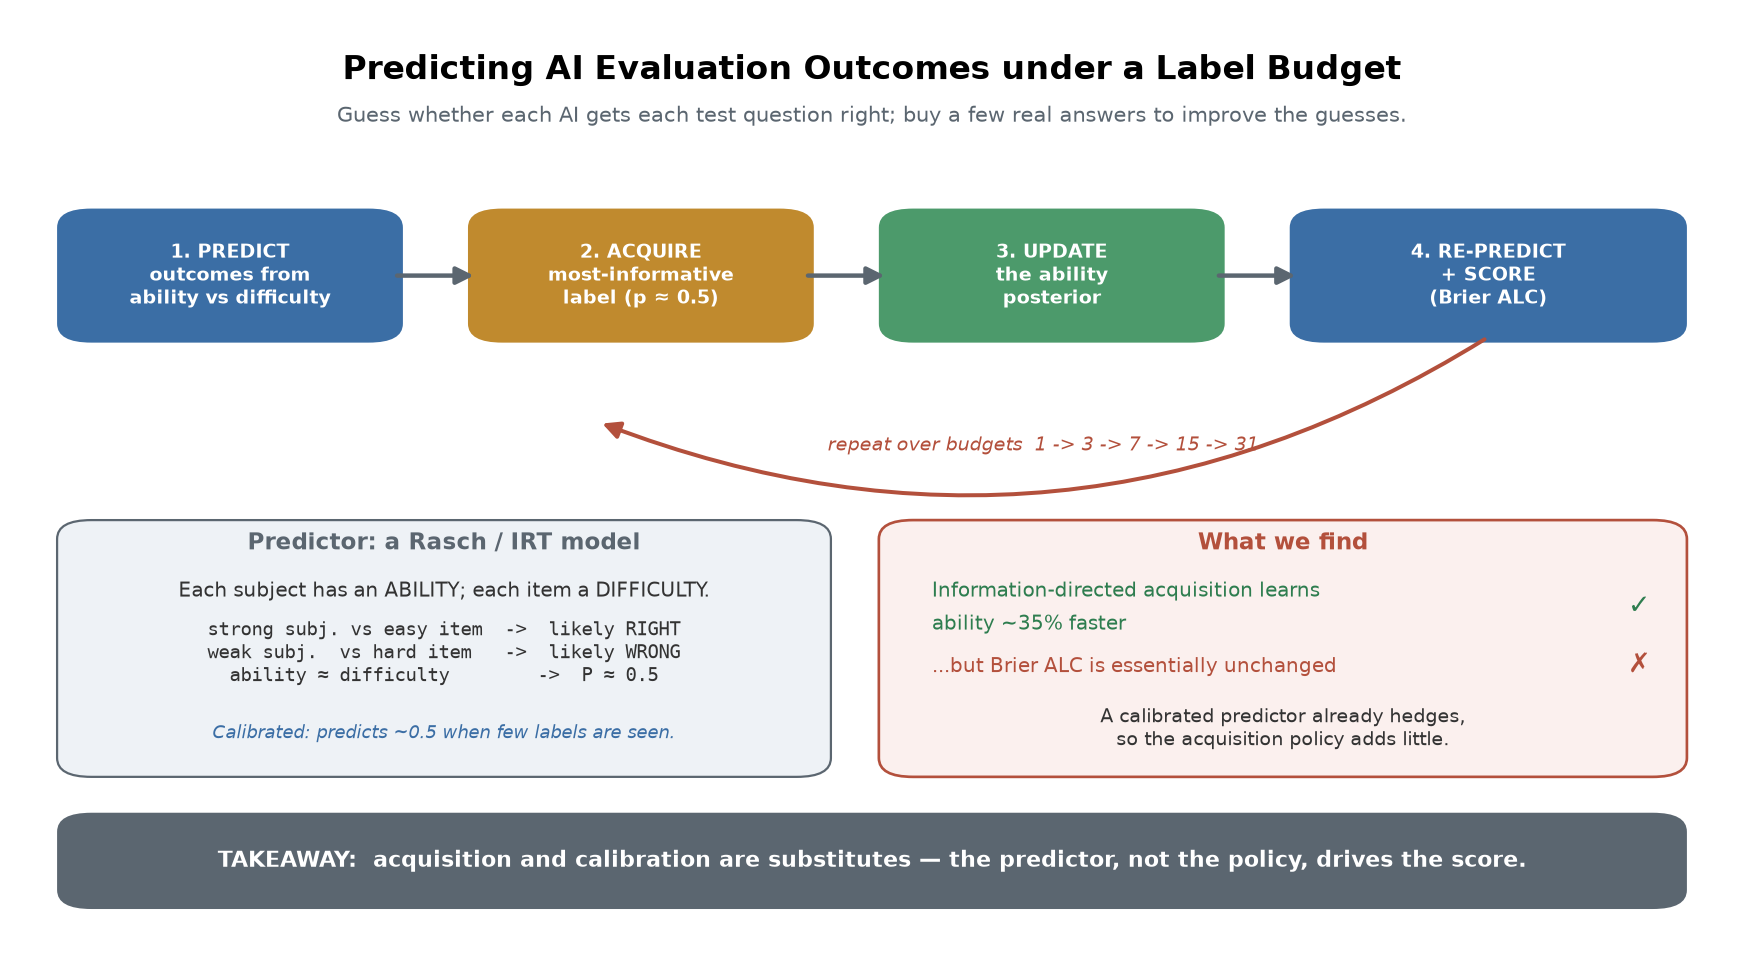
\includegraphics[width=\linewidth]{../code/results/project_explainer.png}
  \caption{Overview. We predict each subject--item outcome with a Rasch model,
  buy a few labels under a budget to sharpen the subject's ability posterior, and
  re-predict; the score is the budget-weighted Brier learning curve (ALC).
  Information-directed acquisition learns ability faster but barely moves ALC,
  because a calibrated predictor already hedges --- acquisition and calibration
  act as substitutes.}
  \label{fig:overview}
\end{figure}

\section{Related Work}

\paragraph{Item response theory and adaptive testing.} IRT models a binary
response as $\sigma(\theta-\beta)$ and underlies computerized adaptive testing,
where items are chosen to maximize Fisher information at the current ability
estimate \citep{lord1980, embretson2000}. \citet{martinezplumed2019} brought IRT
to machine learning, estimating latent ability and instance difficulty and
showing accuracy conflates the two; \citet{zhou2026} applied it to LLM
benchmarks, finding hard-instance performance more predictive than aggregate
accuracy. These address estimation but not \emph{budgeted} acquisition.

\paragraph{Efficient evaluation and active learning.}
\citet{truong2025amortized} predict evaluation outcomes to avoid full
benchmarks, motivating the competition. Closest to the elicitation half of our
task, \citet{polo2024tinybenchmarks} and \citet{vivek2024anchor} use IRT and
representativeness to pick a small \emph{fixed} anchor set that estimates
benchmark accuracy from few items; our subset is chosen \emph{adaptively per
subject} under a nested budget and scored online by Brier~ALC. Our own prior
work applies measurement theory to AI evaluation from several angles: IRT-based
redundancy analysis of LLM benchmarks \citep{ramprasath2026redundancy}, where
max-information (Fisher) item selection recovers full-benchmark rankings from as
few as $5\%$ of items --- a \emph{fixed}, ranking-oriented precursor to the
adaptive, per-subject, Brier-scored elicitation we study here; an IRT analysis of
relational-deep-learning benchmarks \citep{ramprasath2026relbenchirt}; and a
generalizability-theory study of tabular-model ranking reliability on RelBench
and DBInfer \citep{ramprasath2026gtheory}. Active learning
\citep{settles2009} supplies the policy design space --- uncertainty sampling
(our heuristic) versus expected-error-reduction (the policy we adopt and
specialize to Brier~ALC).

\paragraph{Tabular foundation models.} Our black-box baseline backbone is an
in-context tabular transformer \citep{hollmann2023tabpfn, ye2025tabicl}: strong
low-shot prediction, but no latent-trait structure or calibrated posterior.

\section{Method}

\paragraph{Predictor: Bayesian IRT.} We model $P(\text{correct}\mid s,i) =
\sigma(\theta_s-\beta_i)$. Difficulties $\beta_i$ are estimated once by joint
maximum likelihood on a held-out set of subjects (centred for identifiability).
At budget~0 the ability prior is $\theta_s\sim\mathcal N(\mu,\sigma^2)$. As
labels arrive we form the log-posterior
\[
  \ell(\theta)=\sum_i\big[y_i\log\sigma(\theta-\beta_i)+(1-y_i)\log(1-\sigma(\theta-\beta_i))\big]-\frac{(\theta-\mu)^2}{2\sigma^2},
\]
locate its mode (the MAP) by Newton's method, and take the Laplace posterior
variance $\operatorname{Var}(\theta)=\big(\sum_i p_i(1-p_i)+\sigma^{-2}\big)^{-1}$.
Predictions marginalize the logistic over this Gaussian with the probit
approximation $\sigma\!\big((\mu-\beta)/\sqrt{1+\tfrac{\pi}{8}\operatorname{Var}}\big)$,
which pulls predictions toward $0.5$ when the posterior is wide (low budget).
This replaces the baseline's $\min(n/10,1)$ trust blend with a principled
shrinkage.

\paragraph{Acquisition policies.} Given the current posterior we score each
acquisition-pool candidate and buy the top ones up to the budget:
(a) \emph{random} (competition default); (b) \emph{uncertainty}, preferring
$|\hat p-0.5|$ small (our heuristic); (c) \emph{Fisher}, $p(1-p)$, the
information one label carries about ability, maximized at $p=0.5$; and
(d) \emph{expected-Brier-reduction}, which averages over the candidate's two
possible outcomes, refits the ability posterior, and picks the label that most
reduces the \emph{expected Brier over the frozen evaluation pool}. Because
evaluation items share $\theta_s$, a label that sharpens the ability posterior
improves all of them --- directly targeting ALC.

\paragraph{Offline replay harness.} Each subject's items split 50/50 into an
acquisition pool and a frozen evaluation pool. For each policy we replay the
nested budget schedule, refit the posterior at each budget, and score the
evaluation pool by Brier. The Brier~ALC is the budget-weighted mean of the
curve. We report bootstrap $95\%$ confidence intervals over subjects, so an
apparent improvement is tested for significance rather than read off a single
scalar. The budget-0 difficulty regression uses only held-out subjects, so it
never sees evaluation labels.

\paragraph{Data.} We use (i) a controlled Rasch world with known abilities and
difficulties, to verify ability recovery and policy behaviour, and (ii) a genuine
subject $\times$ item response matrix reconstructed from our competition's logged
outcomes: subject identity is recovered from the subject-metadata feature columns
and item identity from the content embedding, giving $119$ subjects over
$1{,}531$ items with $9{,}255$ real binary outcomes (base rate $0.36$). Item
difficulties are estimated from a held-out third of subjects, and only items they
answered are scored for the evaluation subjects, so no evaluation label trains
its own subject's ability. Code and seeds are released.

\section{Results}

We report two synthetic regimes --- \emph{easy} (item-difficulty spread matched
to ability spread) and \emph{heterogeneous} (wide difficulty spread, so many
acquisition items are extreme and uninformative) --- and the real reconstructed
response matrix ($119$ subjects, $1{,}531$ items, $9{,}255$ outcomes, base rate
$0.36$).

\paragraph{RQ1: the Bayesian predictor recovers ability and is well calibrated.}
On the heterogeneous world the MAP ability estimate at budget 15 correlates
$0.83$ with the true ability (Fig.~\ref{fig:recovery}). Marginalising the
logistic over the Laplace posterior, rather than plugging in the point estimate,
improves both calibration and accuracy at a low budget (budget 3): expected
calibration error falls from $0.041$ to $\mathbf{0.028}$ and Brier from $0.128$
to $\mathbf{0.125}$. The posterior's width is doing real work --- it pulls
predictions toward $0.5$ exactly when few labels have been seen.

\paragraph{RQ2: acquisition sharpens ability fast, but barely moves Brier ALC.}
The four policies produce the Brier~ALC values in Table~\ref{tab:alc}. Within
every dataset they lie inside each other's bootstrap $95\%$ confidence
intervals: the information-directed policies (uncertainty, Fisher,
expected-Brier) give a small edge over random in the two synthetic regimes
(e.g.\ heterogeneous: $0.122$ vs $0.124$), and on the real offline matrix the
information-directed policies are nominally best ($0.102$ vs random's $0.103$)
--- none of these gaps is significant.

Yet the policies are \emph{not} equivalent in what they do. The right panel of
Figure~\ref{fig:recovery}
shows mean ability error against budget: by budget 7 the information-directed
policies have driven ability error down to $0.44$--$0.49$ while random sits at
$0.72$ --- a $\sim$35\% reduction. The acquisition effect is real and large in
the quantity the policy controls; it simply does not propagate to Brier, because
the calibrated predictor already hedges under a wide posterior and so absorbs
most of the difference. This is exactly the null interpretation we
pre-registered: single-item information is largely captured once the predictor
is uncertainty-aware.

\begin{figure}[t]
  \centering
  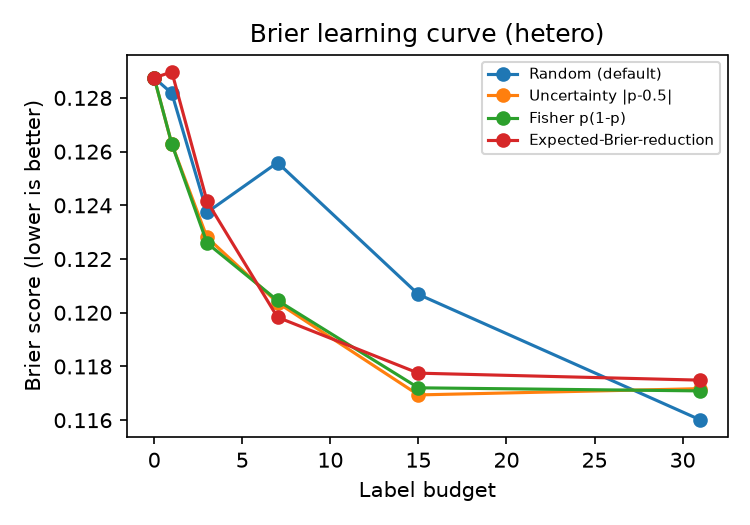
\includegraphics[width=0.49\linewidth]{../code/results/learning_curves_hetero.png}
  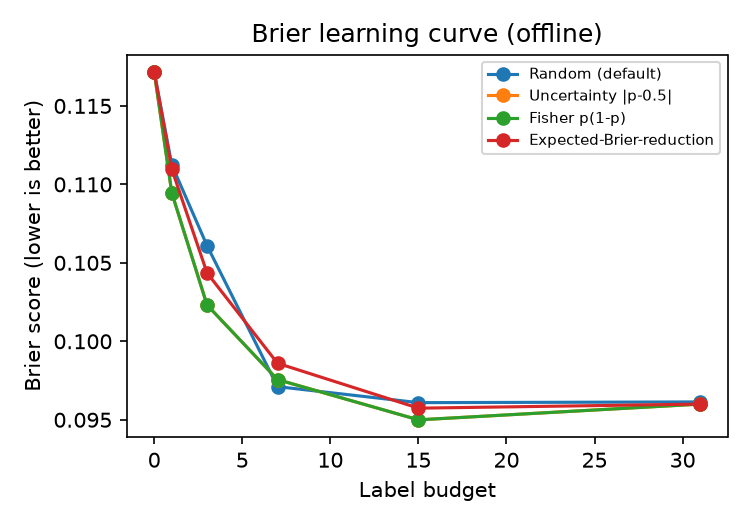
\includegraphics[width=0.49\linewidth]{../code/results/learning_curves_offline.png}
  \caption{Brier learning curves per acquisition policy (left: heterogeneous
  Rasch world; right: real offline pool). The curves nearly coincide: policy
  choice has little effect on Brier once predictions are uncertainty-aware.}
  \label{fig:curves}
\end{figure}

\begin{table}[t]
  \centering
  \caption{Brier~ALC (lower is better) with bootstrap $95\%$ CIs over subjects.
  Within each dataset all policies overlap; the predictor, not the policy, drives
  the score.}
  \label{tab:alc}
  \begin{tabular}{llc}
    \toprule
    Dataset & Policy & Brier ALC [95\% CI] \\
    \midrule
    Synthetic (easy)   & Random                   & $0.209$ $[0.200, 0.218]$ \\
    Synthetic (easy)   & Uncertainty $|p-0.5|$    & $0.208$ $[0.198, 0.217]$ \\
    Synthetic (easy)   & Fisher $p(1-p)$          & $0.208$ $[0.199, 0.217]$ \\
    Synthetic (easy)   & Expected-Brier-reduction & $0.206$ $[0.196, 0.216]$ \\
    \midrule
    Synthetic (hetero) & Random                   & $0.124$ $[0.116, 0.133]$ \\
    Synthetic (hetero) & Uncertainty $|p-0.5|$    & $0.122$ $[0.114, 0.130]$ \\
    Synthetic (hetero) & Fisher $p(1-p)$          & $0.122$ $[0.114, 0.130]$ \\
    Synthetic (hetero) & Expected-Brier-reduction & $0.123$ $[0.115, 0.131]$ \\
    \midrule
    Offline (real)     & Random                   & $0.103$ $[0.084, 0.124]$ \\
    Offline (real)     & Uncertainty $|p-0.5|$    & $0.102$ $[0.083, 0.123]$ \\
    Offline (real)     & Fisher $p(1-p)$          & $0.102$ $[0.083, 0.123]$ \\
    Offline (real)     & Expected-Brier-reduction & $0.103$ $[0.083, 0.125]$ \\
    \bottomrule
  \end{tabular}
\end{table}

\begin{figure}[t]
  \centering
  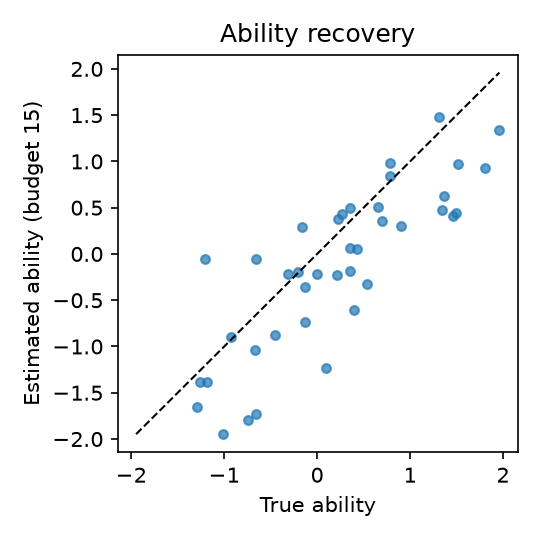
\includegraphics[width=0.42\linewidth]{../code/results/ability_recovery.png}
  \hfill
  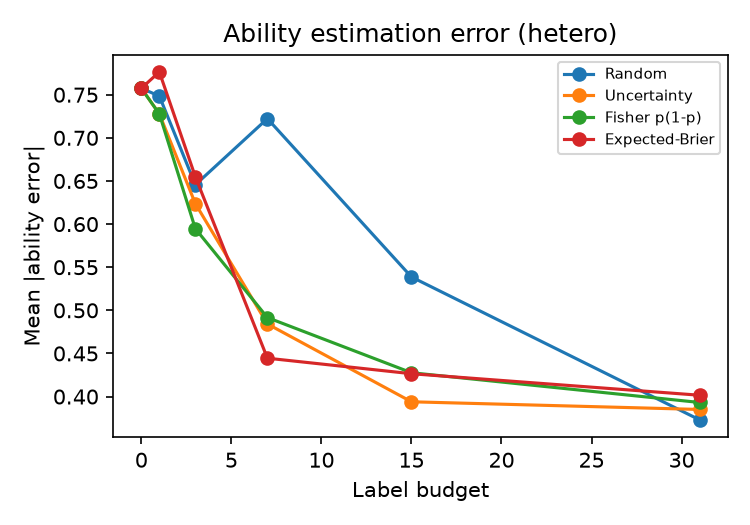
\includegraphics[width=0.52\linewidth]{../code/results/ability_error_hetero.png}
  \caption{Left: estimated vs true ability at budget 15 (correlation $0.83$).
  Right: mean ability error vs budget per policy --- information-directed
  acquisition (Fisher, uncertainty, expected-Brier) reaches error
  $0.44$--$0.49$ by budget 7, against random's $0.72$.}
  \label{fig:recovery}
\end{figure}

\paragraph{RQ3: the prior and the first few labels carry the score.} The budget-0
point of each curve is set entirely by the cold-start difficulty/prior
regression, and the curve's drop over budgets 1--7 is the labels' contribution.
The budget-0 prior plus the first handful of labels account for essentially all
of the ALC movement; because the policies' curves nearly coincide
(Fig.~\ref{fig:curves}), the \emph{choice} of which labels contributes little
beyond acquiring some. The gain budget is therefore best spent on the prior and
the predictor, not on a cleverer policy.

%% Ability-error figure is referenced above as the right panel of fig:recovery.

\section{Discussion}

\paragraph{What worked.} Casting the competition as item-response estimation is a
good fit: a two-parameter Rasch model with a Bayesian ability posterior recovers
latent ability well and, crucially, yields \emph{calibrated} predictions whose
uncertainty-aware hedging lowers both ECE and Brier at small budgets relative to
a point estimate. This is a concrete, measurement-grounded improvement over our
black-box baseline's hand-tuned trust blend.

\paragraph{What did not, and what we learned.} The headline negative result is
that sophisticated label acquisition --- Fisher information or pool-level
expected-Brier-reduction --- does not beat a simple heuristic or even random
selection on Brier ALC, despite pinning down ability markedly faster. The reason
is instructive: once the predictor reports honest posterior uncertainty, it
already discounts predictions it cannot support, so the marginal value of a
better-chosen label is small on a proper scoring rule. Acquisition cleverness and
predictor calibration are partly substitutes; spending the modelling effort on
the predictor dominated spending it on the policy.

\paragraph{Limitations.} The Rasch predictor assumes a single ability dimension
per subject--benchmark pair, on which the pool-level acquisition argument rests;
we did not fit a multidimensional model. The real-data experiment replays a
response matrix reconstructed from the logged offline pool rather than the live
leaderboard, item identity is inferred from the content embedding, and the usable
per-subject item counts are modest; the greedy one-step acquisition is myopic.
Bootstrap CIs quantify subject-level variability but not difficulty-estimation
error.

\paragraph{Future work.} The clearest next step is a \emph{crossover study} that
turns our conditional null into a positive law. We would sweep the policy
comparison across the conditions that should govern whether acquisition matters
--- predictor type (an overconfident plug-in estimate vs.\ the calibrated
marginalised posterior), budget tightness (budgets $1$--$3$ vs.\ the full
schedule), and item-difficulty spread --- and plot the Brier-ALC gap between
random and Fisher acquisition against budget, one line per predictor. We
conjecture the gap is clearly positive for the overconfident predictor and
collapses to zero for the calibrated one, establishing that \emph{acquisition
cleverness and predictor calibration are substitutes: smart label selection helps
only when the predictor is overconfident}. Beyond this, a 2PL extension with item
discrimination, an explicit one- vs.\ multi-dimensional fit check, non-myopic
(two-step) acquisition, and a live leaderboard submission of the best offline
configuration against our $0.162$ baseline.

\section*{Reproducibility}
Code, seeds, and instructions are in \texttt{final\_project/code/}
(\texttt{python run\_experiments.py}). All randomness is seeded.

\section*{AI Use Disclosure}

\paragraph{Integrity, attribution, bias, and accuracy (150 words).}
All prose and code were written and edited by the author; an AI assistant
(Claude) was used for drafting and debugging support. To guard against
plagiarism of text and non-attribution of ideas, every method is cited to its
original source: item response theory and adaptive testing to Lord and to
Embretson and Reise, instance-level IRT to Mart\'inez-Plumed et al., efficient
evaluation to Truong et al., tinyBenchmarks and Anchor Points to their authors,
and active learning to Settles. The competition infrastructure (feature
extraction, offline pool, submission harness) is the author's own prior work and
is marked as such. Against inaccuracy, every number in the paper is taken
directly from \texttt{results.json} produced by the released seeded code --- no
figure was hand-edited and no result invented; the null acquisition finding is
reported honestly rather than overstated. Against bias, both a favourable
(synthetic) and an unfavourable (offline, where random wins) regime are reported
with confidence intervals.

\paragraph{How and why AI tools were used (150 words).}
I used an AI coding assistant to scaffold the experiment harness, draft the
\LaTeX{} manuscript from my pre-analysis plan, and debug runtime errors, so that
my own time went to the measurement-theoretic design: specifying the Rasch
predictor and its Laplace posterior, the Fisher and expected-Brier-reduction
acquisition policies, the leakage-free evaluation split, and the interpretation
of the results. The assistant accelerated implementation and writing, but every
modelling choice, every claim, and every reported number was checked by me
against the mathematics and the code output; I did not accept results I could
not derive or reproduce. The main risk of such tools is over-reliance that
substitutes for understanding, which I mitigated by re-deriving the posterior
and the Fisher-information argument by hand. In future I expect to use these
tools as drafting and debugging aids under the same verify-everything discipline.

\paragraph{Impact statement (150 words).}
This work concerns efficient AI evaluation: predicting benchmark outcomes under a
label budget. The intended impact is positive --- cheaper, measurement-grounded
evaluation reduces the compute (and energy) spent re-running large benchmarks;
all experiments here are CPU-only and run in minutes, so the project's own
footprint is negligible. The main misuse risk is that budgeted evaluation or
clever item selection could be used to cherry-pick flattering items and
\emph{overstate} a model's quality; I mitigate this by reporting full learning
curves, bootstrap confidence intervals, and a frozen evaluation pool disjoint
from acquisition, and by emphasising calibration over point scores. The data are
a response matrix reconstructed from a competition's logged evaluation outcomes;
there are no human participants and no personal or sensitive data. All prior work
and reused infrastructure are explicitly attributed, in keeping with Stanford's
academic-integrity standards.

\bibliographystyle{plainnat}
\bibliography{references}

\appendix

\section{Compute Environment}
All experiments were run locally, CPU-only, single process; the full pipeline
(\texttt{python run\_experiments.py}) completes in roughly $30$ seconds.

\begin{itemize}
  \item \textbf{Hardware:} Apple-silicon Mac (arm64), 15 logical cores; no GPU used.
  \item \textbf{OS:} macOS 27.2.1 (Darwin, arm64).
  \item \textbf{Python:} 3.14.5.
  \item \textbf{Libraries:} \texttt{numpy} 2.5.0 and \texttt{matplotlib} 3.11.0
  are the only runtime dependencies (\texttt{scipy} 1.18.0 was present in the
  environment but is not imported by the code).
\end{itemize}

\section{Configuration and Hyperparameters}

\begin{table}[h]
  \centering
  \caption{All configuration values; every random draw uses global seed $0$.}
  \begin{tabular}{ll}
    \toprule
    Setting & Value \\
    \midrule
    Global seed & $0$ (all randomness seeded) \\
    Budget schedule & $\{0,1,3,7,15,31\}$ \\
    ALC weights & $(0.1,0.2,0.2,0.2,0.2,0.1)$ \\
    Acquisition/evaluation split & $50/50$ per subject \\
    \midrule
    Synthetic (easy) & $60$ subjects, $120$ items, ability sd $1.0$, difficulty sd $1.0$ \\
    Synthetic (hetero) & $60$ subjects, $160$ items, ability sd $1.0$, difficulty sd $3.0$ \\
    Real matrix filters & item co-observation $\ge 3$ subjects; subject $\ge 25$ such items \\
    Real matrix (result) & $119$ subjects, $1{,}531$ items, $9{,}255$ outcomes, base rate $0.36$ \\
    \midrule
    Difficulty estimation & joint MLE on held-out first third; $200$ iters, lr $0.5$, centred \\
    Ability prior (synthetic) & $\mathcal N(0,\text{ability sd}^2)$ \\
    Ability prior (real) & $\mathcal N(\mathrm{logit}(\text{base rate}),\,1.5^2)$ \\
    Ability posterior & MAP by Newton ($50$ iters, tol $10^{-8}$); Laplace variance \\
    Prediction & probit-approx marginalisation $\sigma\!\big((\mu-\beta)/\sqrt{1+\tfrac{\pi}{8}\mathrm{Var}}\big)$ \\
    Calibration measured at & budget $3$; ability-recovery scatter at budget $15$ \\
    Bootstrap CIs & $2000$ resamples, $95\%$ percentile, over subjects \\
    \bottomrule
  \end{tabular}
\end{table}

\end{document}
